\section{Black Scholes Construction}

Consider a financial security such as a stock $S$ with current market price $S_0$. At some future time $T$ let the price of $S$ be represented by a random variable $S_T$ whose probability distribution is indicated in figure \ref{fig:S_T}. Here, no presumption is yet made about the kind of distribution for $S_T$. 

\begin{figure}
  \centering
  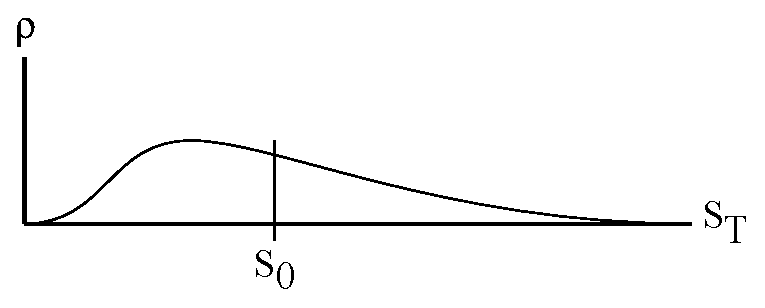
\includegraphics[width=2.5in]{Images/S_T.eps}
  \caption[Distribution of Stock Prices at time T]
          {Distribution of $S_T$}
  \label{fig:S_T}
\end{figure}

Following Dineen \cite{dineen00} suppose now that $S_T$ satisfies the so-called \emph{no-arbitrage requirement} $S_0 = \mathbb{E}[S_T]$. Suppose an investor, Ivan, holds one unit of stock $S$ as the sole content of his portfolio of assets. Initially his wealth $W$ is then just,

\begin{align*}
W_0 = S_0
\end{align*}

and at time $T$ his wealth is expressed as,

\begin{align*}
W_T = S_T
\end{align*}

Expressing Ivans future wealth in terms of his current wealth and a continuously compounding growth rate $r$ one writes

\begin{align*}
W_T = W_0 e^{r_T}
\end{align*}

where

\begin{align*}
r_T = log(\frac{S_T}{S_0}).
\end{align*}

Referring to $\hat{S_T} = S_T / S_0$ as the \emph{normalized} stock price rescale the probability distribution $S_T$ to $\hat{S_T}$ so that the mean of $\hat{S_T}$ is one as depicted in figure \ref{fig:S_T_hat}.

\begin{figure}
  \centering
  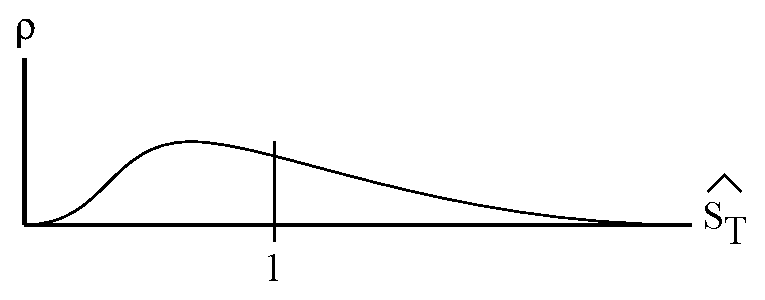
\includegraphics[width=2.5in]{Images/S_T_hat.eps}
  \caption[Distribution of Normalized Stock Price at time T]
          {Distribution of $\hat{S_T}$}
  \label{fig:S_T_hat}
\end{figure}

Since $r_T$ is the log of $\hat{S_T}$, its mean is zero as illustrated in figure \ref{fig:r_T}. Notice that if $\hat{S_T}$ is represented by a LogNormal random variable then $r_T$ is represented by a Normal random variable with zero mean.

\begin{figure}
  \centering
  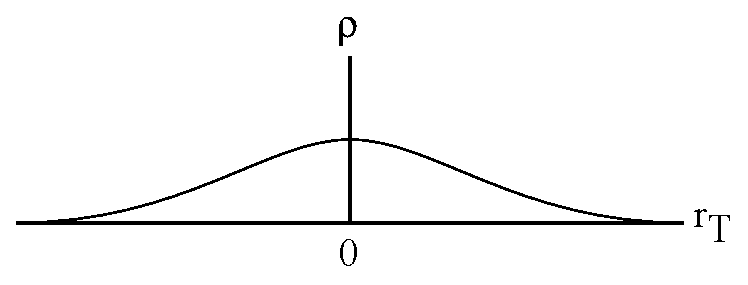
\includegraphics[width=2.5in]{Images/r_T.eps}
  \caption[Distribution of Return Rate at time T]
          {Distribution of $r_T$}
  \label{fig:r_T}
\end{figure}

If instead of holding a unit of stock $S$, the investor Ivan holds a European-style call option $C$ based on stock $S$ with strike price $K$ exercisable at time $T$. The value of $C$ at time $T$ is given by

\begin{align*}
C_T = [S_T - K]^+
\end{align*}

similarly, the related put-option $P$ with the same parameters as $S$ has value $P_T$ at time $T$ with

\begin{align*}
P_T = [S_T - K]^-
\end{align*}

It is helpful to notice that $C_T, P_T \ge 0$. For ease of calculation, the assumption is made that upon maturity all options are settled in cash and that there is no requirement that the \emph{underlying} stock be transferred between parties. A further assumption made here is that all cash values are stated in current (t = 0) dollars. Please note that this runs counter to the not uncommon practice in financial texts, e.g. \cite{dineen00} to include the effect of time-value-of-money in calculations. While the current dollars assumption is equivalent to zero interest rate, the understanding is that all cash may be restated in any chosen year denomination.

To find the probability distribution over the mature value $C_T$ of the call option $C$ at time $T$ with the underlying stock $S$ and strike price $K$, a sequence of transformations of $S_T$ are necessary. The first transformation is to subtract the strike price $K$ from the distribution $S_T$. The resulting distribution is illustrated in figure \ref{fig:S_T_minus_K}. The key feature is represented by the shaded region in figure \ref{fig:S_T_minus_K} is the probability $q$, such that $q = Pr\{S_T - K \le 0\}$. 

\begin{figure}
  \centering
  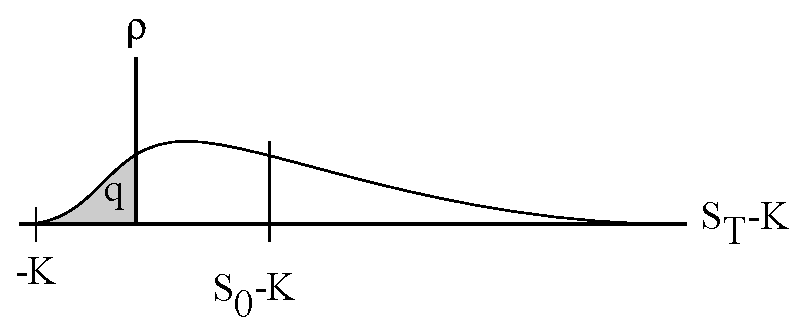
\includegraphics[width=2.5in]{Images/S_T_minus_K.eps}
  \caption[Distribution of $S_T$ Minus Strike Price $K$]
          {Distribution of $S_T - K$}
  \label{fig:S_T_minus_K}
\end{figure}

The second transformation, the probability distribution of $[S_T - K]^+$ is illustrated in figure \ref{fig:S_T_minus_K_plus}. Notice that the probability $q$ is now concentrated discretely at zero and represented by a vertical arrow labeled $q$. Since the remaining portion of the distribution is continuously distributed, the vertical axis still represents probability density. Notice further that the mean $\mu_{C_T}$ of this mixed, continuous/discrete probability distribution, is indicated at some positive location in figures. Notice that as $C_T = [S_T - K]^+$,

\begin{align*}
\mu_{C_T} = \mathbb{E}[[S_T - K]^+] = \mathbb{E}[C_T]
\end{align*}

The significance of $\mu_{C_T}$ in figure \ref{fig:S_T_minus_K_plus} is that this price, based on the no-arbitrage principle, an investor can expect to pay today $(t = 0)$ for a call of this type when $S_T$ represents the commonly accepted probability distribution of the value of stock $S$ at time $T$. That is,

\begin{align*}
C_0 = \mu_{C_T} = \mathbb{E}[C_T]
\end{align*}

\begin{figure}
  \centering
  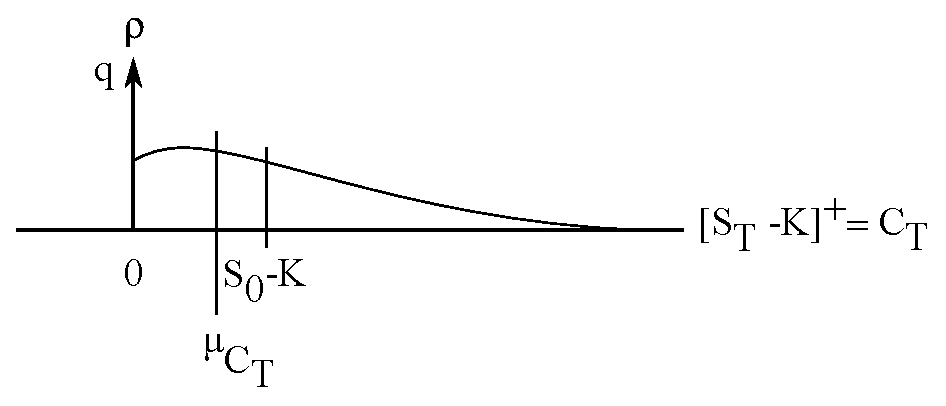
\includegraphics[width=2.5in]{Images/S_T_minus_K_plus.eps}
  \caption[Distribution of Positive Portion of $S_T$ Minus Strike Price $K$]
          {Distribution of $[S_T - K]^+$}
  \label{fig:S_T_minus_K_plus}
\end{figure}

Normalizing the distribution of the mature call option with respect to the initial value of the underlying $S_0$ gives the distribution for $\hat{C_T}$, the normalized call option price, illustrated in figure \ref{fig:C_T_hat}.

\begin{figure}
  \centering
  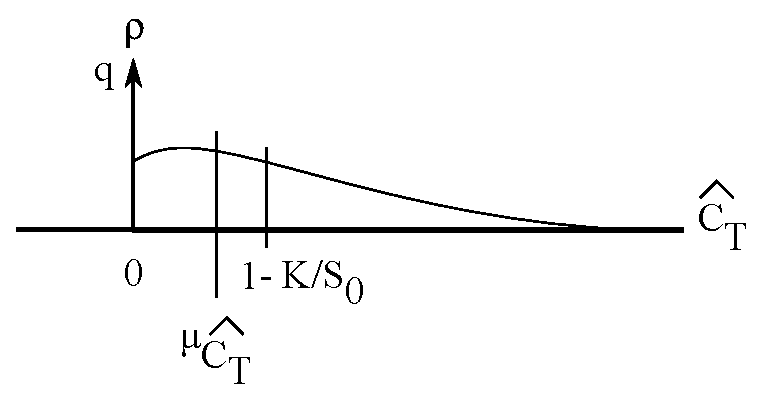
\includegraphics[width=2.5in]{Images/C_T_hat.eps}
  \caption[Distribution of Normalized Mature Call]
          {Distribution of $\hat{C_T}$}
  \label{fig:C_T_hat}
\end{figure}

Using the same strike price $K$ and underlying stock $S$, a put option value at maturity is illustrated in figure \ref{fig:S_T_minus_K_minus} where value at maturity of the put option is,

\begin{align*}
P_T = \mathbb{E}[[S_T - K]^-]
\end{align*}

and the no-arbitrage price of the put is,

\begin{align*}
P_0 = \mu_{P_T}
\end{align*}

Note that the probability concentrated at zero here is $1-q = Pr\{S_T - K < 0\}$.

\begin{figure}
  \centering
  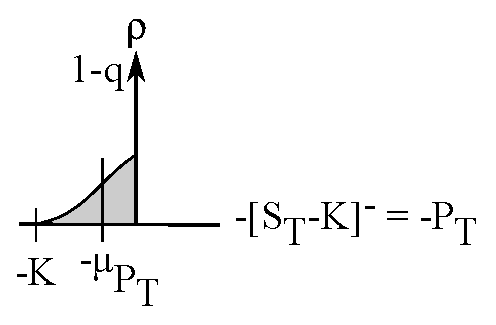
\includegraphics{Images/S_T_minus_K_minus.eps}
  \caption[Distribution of Negative Portion of $S_T$ Minus Strike Price $K$]
          {Distribution of $-[S_T - K]^-$}
  \label{fig:S_T_minus_K_minus}
\end{figure}

The \emph{put-call parity formula},

\begin{align*}
\mathbb{E}[C_T] - \mathbb{E}[P_T] = S_0 - K
\end{align*}

is now obtained easily using the notation stated above, noting that

\begin{align*}
\mathbb{E}[C_T] - \mathbb{E}[P_T] &= S_0 - K\\
\mathbb{E}[C_T - P_T] &= S_0 - K\\
\mathbb{E}[[S_T - K]^+ - [S_T - K]^-] &= S_0 - K\\
\mathbb{E}[S_T - K] &= S_0 - K\\
\mathbb{E}[S_T] - K &= S_0 - K\\
S_0 - K &= S_0 - K\\
\end{align*}

as in Dineen \cite{dineen00}, with the exception that Dineen \cite{dineen00} denotes as $C_T$ the expected value of the probability distribution denoted $C_T$ in this paper and similarly for $P_T$. 

There is a geometric interpretation of Put-Call Parity. This can be seen in the perspective figure \ref{fig:CP_addition}, where the probability density axis is perpendicular to the $C_T \times (−P_T)$-space. Put–Call Parity is realized in that figure as the elementary projection of the joint $C_T \times (−PT)$-space to the diagonal $C_T + (−P_T)$-space. The analogous algebraic calculation procedure is detailed in the appendix.

\begin{figure}
  \centering
  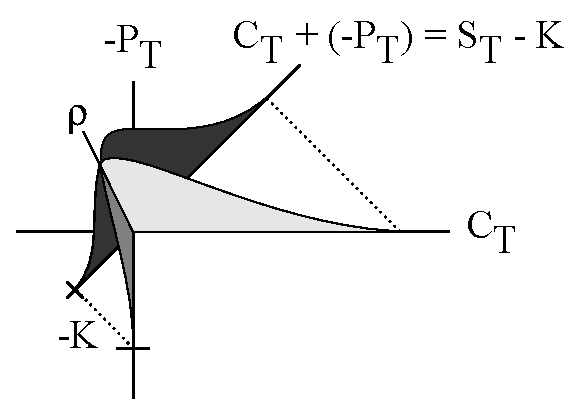
\includegraphics[width=3in]{Images/CP_addition.eps}
  \caption[Distribution of Put-Call Parity in Perspective]
          {Distribution of $C_T - P_T = S_T - K$ in Perspective}
  \label{fig:CP_addition}
\end{figure}

%%%%%%%%%%%%%%%%%%%%%%%%%%%%%%%%%%%%%%%%%%%%%%%%%%%%%%%%%%%%%%%%%%%%%%%%%%%%%%%%%%%%%%%%%%%%%%%

\subsection{Geometric Black-Scholes Pricing}

Suppose now that a random variable $X$ has probability density function $\rho(x)$ and is ``well behaved'' enough to have mean $M = \mathbb{E}[X] < \infty$. Suppose further we have a partition point $K$ as shown in figure \ref{fig:S_T_K_generic} and let $q = Pr\{X < K\}$ and so $1 - q = Pr\{X \ge K\}$.

\begin{figure}
  \centering
  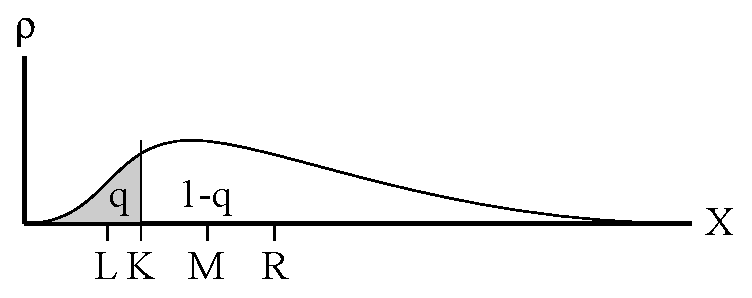
\includegraphics[width=2.5in]{Images/S_T_K.eps}
  \caption[Probability Distribution Partitioned at $K$]
          {Probability Distribution Partitioned at $K$}
  \label{fig:S_T_K_generic}
\end{figure}

Form two new \emph{truncated} random variables from the left and right sections of the $K$-partitioned random variable $X$ with probability densities,

\begin{align*}
X_L \sim \rho_L(x) &= \frac{\rho(x) \mathbf{1}_{X < K}}{q}\\
X_R \sim \rho_R(x) &= \frac{\rho(x) \mathbf{1}_{X \ge K}}{1-q}
\end{align*}

\begin{figure}
  \centering
  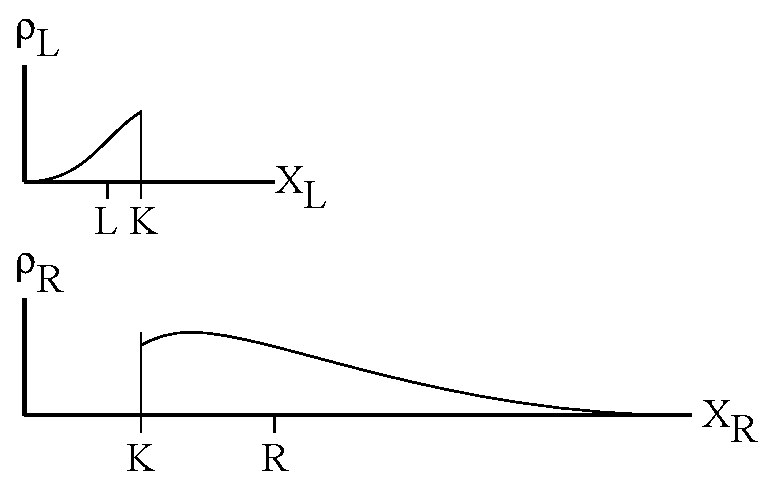
\includegraphics{Images/XL_XR.eps}
  \caption[Left- and Right-Truncated Random Variables]
          {Left- and Right-Truncated Random Variables}
  \label{fig:XL_XR}
\end{figure}

as depicted in figure \ref{fig:XL_XR} where the $L$ and $R$ are expected values of $X_L$ and $X_R$. Notice that the affine combination of $L$ and $R$ via $q$, illustrated in figure \ref{fig:XL_XR_M}, yields the original mean $M$,

\begin{align*}
M = q * L + (1-q) * R
\end{align*}

\begin{figure}
  \centering
  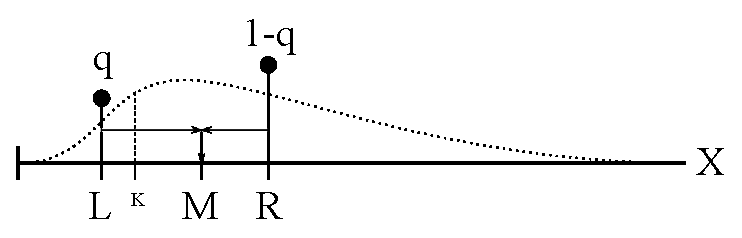
\includegraphics{Images/XL_XR_M.eps}
  \caption[Mean Relationship Between Bifurcated Sections]
          {Mean Relationship Between Bifurcated Sections}
  \label{fig:XL_XR_M}
\end{figure}

Toward Geometric Black-Scholes pricing define new random variables $Y = K + [X-K]^+$ and $Z$, a discrete random variable such that $Pr\{Z = K\} = 1$ with discrete density $\rho_Z = \mathbf{\delta}_{z = K}$. Then the density $\rho_Y$ of $Y$ is

\begin{align*}
\rho_Y(y) = q * \rho_z(y) + (1-q) * \rho_R(y)
\end{align*}

and depicted in figure \ref{fig:Z_XR_K}. Note in particular that $Y$ is a \emph{mixed} discrete and continuous random variable.

\begin{figure}
  \centering
  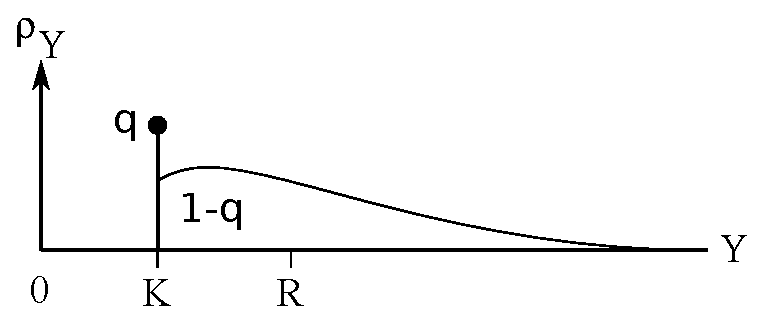
\includegraphics[width=2in]{Images/Z_XR_K.eps}
  \caption[Positive Density]
          {Positive Density}
  \label{fig:Z_XR_K}
\end{figure}

To compute the mean of $Y$, the $X_R$ portion of $Y$ may be replaced with a discrete density $(1-q)$ at the mean $R$ of $X_R$, as illustrated in figure \ref{fig:Z_XR_K_discrete}. The mean $M_Y$ of $Y$ is then the affine combination

\begin{align*}
M_Y = \mathbb{E}[Y] = q * K + (1-q) * R
\end{align*}

\begin{figure}
  \centering
  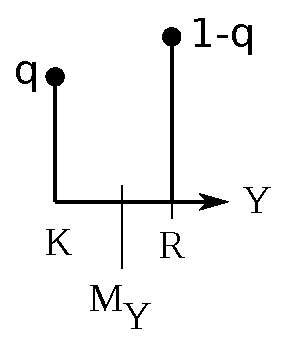
\includegraphics[width=0.75in]{Images/Z_XR_K_discrete.eps}
  \caption[Geometric Black-Scholes Pricing]
          {Geometric Black-Scholes Pricing}
  \label{fig:Z_XR_K_discrete}
\end{figure}

Finally Geometric Black-Scholes pricing requires computing the mean of $[X-K]^+$ for some random variable $X$ such that $\mathbb{E}[X] < \infty$ and constant $K$. Using the notation developed in this section the result is expressed immediately as

\begin{align*}
\mathbb{E}[[X-K]^+] &= \mathbb{E}[Y] - K
\end{align*}

and more conveniently as,

\begin{align*}
\mathbb{E}[[X-K]^+] + K &= q * K + (1-q) * R
\end{align*}

As an illustrative example the traditional Black-Scholes formula is recovered by letting $X = S_T$ be a LogNormally distributed random variable representing the stock price of the underlying asset at some future time $T$. To use Geometric Black-Scholes to price a European-style call option with maturity time $T$ and strike price $K$ let $C_T = [X-K]^+$ and find the current price of the call option as $C_0 = \mathbb{E}[C_T]$. Following the steps above symbolically first identify the probability density of $S_T$,

\begin{align*}
\rho(x) = \frac{1}{x \sqrt{2 \pi} \sigma} e^{-\frac{1}{2}(\frac{ln(x) - \mu}{\sigma})^2}
\end{align*}

Following Dineen \cite{dineen00}, the current price $S_0$ is the mean of $S_T$,

\begin{align*}
S_0 = \mathbb{E}[S_T] = e^{\mu + \frac{\sigma^2}{2}}.
\end{align*}

Since $S_0$ is a known quantity it may be used to solve for the unknown LogNormal parameter $\mu$,

\begin{align*}
\mu = ln(S_0) - \frac{\sigma^2}{2}
\end{align*}

and the parameter $\sigma$, according to standard interpretations, e.g. Dineen \cite{dineen00}, represents the asset volatility and must be given. The option price $C_0$ is expressed by the formula derived above as

\begin{align*}
C_0 + K &= q * K + (1-q) * R\\
C_0 &= (1-q) * R - (1-q) * K
\end{align*}

Finding the mean $R$ of the right-truncated LogNormal and its associated probability $(1-q)$,

\begin{align*}
R &= \frac{1}{1-q}\frac{1}{\sqrt{2 \pi} \sigma} \int_K^\infty e^{-\frac{1}{2}(\frac{ln(x) - \mu}{\sigma})^2} \; dx\\
&= \frac{1}{1-q} e^{\mu + \sigma^2 / 2} \Phi\left(\frac{-ln(K) + \mu + \sigma^2}{\sigma}\right)\\
&= \frac{1}{1-q} S_0 \Phi\left(\frac{ln(S_0/K) + \sigma^2 / 2}{\sigma}\right)
\end{align*}

and

\begin{align*}
1-q &= \Phi\left(-\frac{ln(K)-\mu}{\sigma}\right)\\
    &= \Phi\left(\frac{ln(S_0 / K) - \sigma^2 / 2}{\sigma}\right)
\end{align*}

where

\begin{align*}
\Phi(z) &= Pr(Z <= z) \; \text{ for } Z \sim Normal(\mu, \sigma^2)
\end{align*}

the traditional Black-Scholes formula follows immediately,

\begin{align*}
C_0 &= S_0 \Phi\left(\frac{ln(S_0 / K) + \sigma^2 / 2}{\sigma}\right) - K \Phi \left(\frac{ln(S_0 / K) - \sigma^2 / 2}{\sigma}\right)
\end{align*}

\subsection{Portfolio Construction}

Given a stock $S$ represented at time $t=0$ by value $S_0$ and at $t=T$ by random variable $S_T$ and a European call option $C$ based on $S$ with strike price $K$ at time $T$ the domain of the joint probability distribution of $S$ and $C$ is shown in figure \ref{fig:SC}. The point $(S_0, C_0)$ corresponds to the joint initial price of the stock and call. The broken line is the familiar curve for a call option graph. Perpendicular to the $SC-plane$ is the joint probability density of $S$ and $C$ at time $T$. The probability density is zero at points away from the broken line.

\begin{figure}
  \centering
  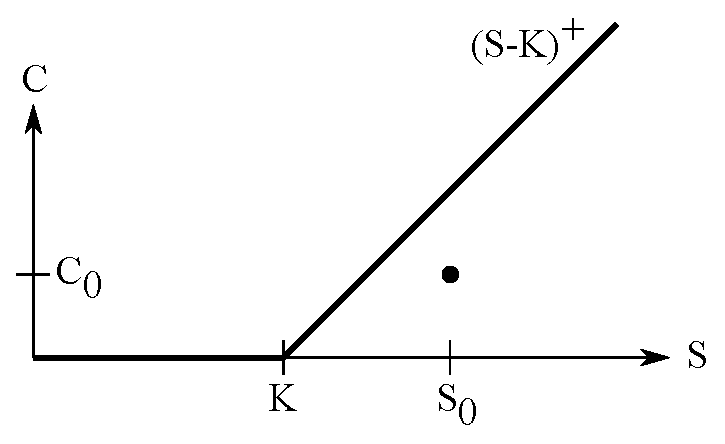
\includegraphics[width=3in]{Images/SC.eps}
  \caption[Stock-Call Space]
          {Stock-Call Space}
  \label{fig:SC}
\end{figure}

Since the $SC$-space represents the price per unit of each financial security there is a dual space where each point represents the number of units held in a hypothetical portfolio. This dual space is referred to here as the portfolio space. Given a portfolio vector $\pi$ and a point $w$ in $SC$ the dollar value of $pi$ at $w$ is $\pi^T\;w$. Recall that the projection matrix of $SC$ onto a vector $v$ in $SC$ is given by,

\begin{align*}
\Pi = \frac{v\;v^T}{v^T\;v}
\end{align*}

Notice that given portfolio $\pi = (\pi_s, \pi_c)$ the random variable $Z_T = \pi_s * S_T + \pi_c * C_T$ appears graphically as a hyperplane in $SC$-space. Notice in particular that if the projection vector in $SC$-space is $\pi$ itself then the projection matrix becomes,

\begin{align*}
\Pi = \frac{\pi\;\pi^T}{\pi^T\;\pi}
\end{align*}

and more to the point the portfolio value $V$ given $x \in SC$-space is,

\begin{align*}
V &= \pi^T\;x\\
  &= \pi^T \frac{\pi\;\pi^T}{\pi^T\;\pi} x\\
  &= \pi^T \Pi x
\end{align*}

which means the value of a portfolio, $\pi$, may be visualized by representing $\pi$ as a vector in $SC$-space, projecting any other point in $SC$ space orthogonally onto $\pi$ and then computing the inner product of $\pi$ and the projected point to find the portfolio value. 

Suppose, for example, $\pi = (2,1)$, that is the portfolio contains two shares of stock and one call option with strike price $K$. The initial price of the stock is $S_0$ and the initial price of the call is $C_0$ as usual. This situation is depicted in figure \ref{fig:SC_21}. The portfolio is represented by $Z$, the linear combination of $S$ and $C$. Notice that if $S_T = 0$ then $Z = 0$. If $S_T = K$ then $Z = 2K$ since the call expires out-of-the-money and the value of the portfolio reflects the two shares of stock alone. Geometrically the $Z=2K$ is found by orthogonally projecting the point $(K,0)$ to the $\pi = (2,1)$ vector (the $Z$-line) and measuring the result with the dual vector, also $\pi$ to find $V = 2*K + 1*0$. The initial value of the portfolio is shown graphically as $Z_0$ which is consistent with the computed value of $Z_0 = 2*S_0 + 1*C_0$. This construction is consistent with the understanding that random variables are represented in a joint space and observed individually through projection. 

\begin{figure}
  \centering
  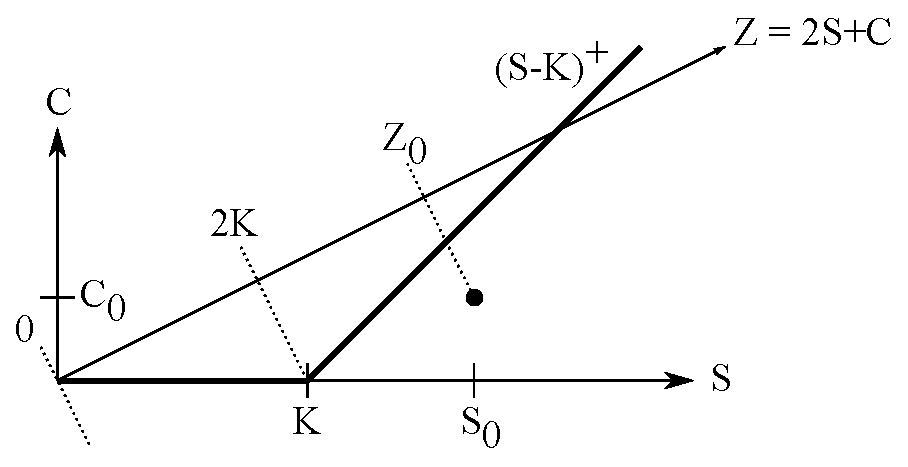
\includegraphics[width=3in]{Images/SC_21.eps}
  \caption[Stock-Call Space with (2,1) Portfolio]
          {Stock-Call Space with (2,1) Portfolio}
  \label{fig:SC_21}
\end{figure}

Orthogonal projection implies the existence of a null space hyperplane. A natural construction is that of a portfolio whose initial value lies in this null space. The initial cost of such a portfolio is zero. Suppose that a call option with strike price $K$ costs $C_0$ with underlying stock of initial cost $S_0$ and that $S_0 / C_0 = 5$, for example. A zero-cost portfolio is $\pi = (-1,5)$, that is, sell one share of stock and buy $5$ call options. This situation is depicted in figure \ref{fig:SC_Zero}. The zero-cost portfolio is represented by $Z = -S + 5C$. Notice that $min(Z) = -K$ and that if the final stock price $S_T$ is $2K$ instead of $K$ the value of the portfolio $Z$ jumps from $-K$ to $3K$, four multiples of $K$ since the portfolio contains $5$ calls and one shorted share of stock whereas the terminal stock price rising form $0$ to $K$ results in $Z$ falling from $0$ to $-K$ since it contains the shorted stock and $5$ out-of-the-money call options. 

The probability distribution of the example $Z$ is approximated in figure \ref{fig:SC_Zero_RV} where the negative-put-like behavior is shaded and marked with its total probability $q$ assuming $S_T$ is represented by a $LogNormal$ random variable. Notice in particular that the probability distribution of $Z$ is not recognizable as either $LogNormal$ nor truncated $LogNormal$.

\begin{figure}
  \centering
  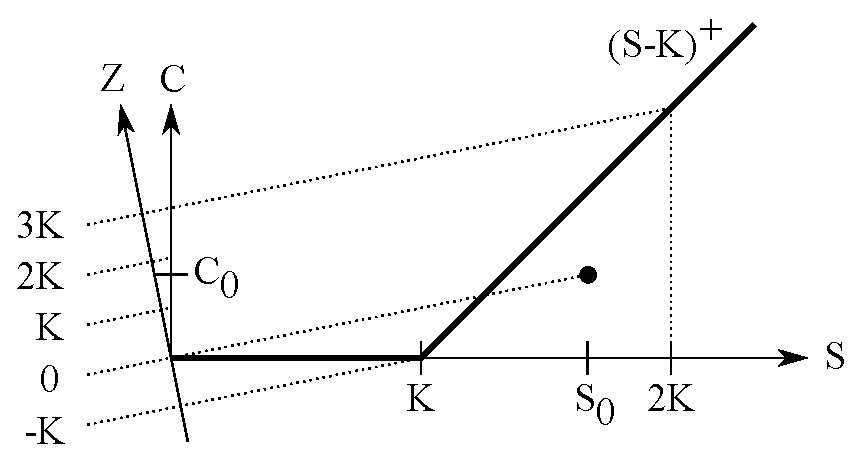
\includegraphics[width=3in]{Images/SC_Zero.eps}
  \caption[Stock-Call Space with Zero-Cost Portfolio]
          {Stock-Call Space with Zero-Cost Portfolio}
  \label{fig:SC_Zero}
\end{figure}

\begin{figure}
  \centering
  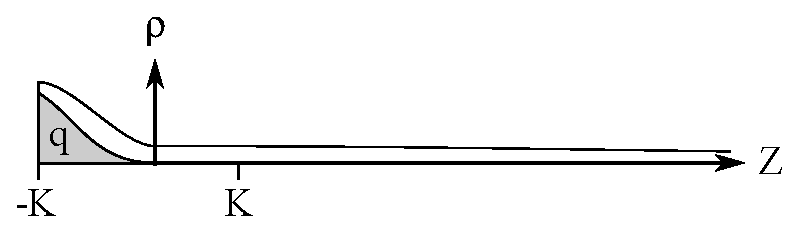
\includegraphics[width=3in]{Images/SC_Zero_RV.eps}
  \caption[Probability Distribution of Zero-Cost Portfolio]
          {Probability Distribution of Zero-Cost Portfolio}
  \label{fig:SC_Zero_RV}
\end{figure}

\subsection{Black Scholes Construction: SPY Example}

The work on Levy-Stable distributions by Nolan \cite{nolan13} takes the daily prices of a particular stock (ticker: SPY) shown in figure \ref{fig:SPY}. The daily returns for SPY are plotted in figure \ref{fig:SPY_returns}.

\begin{figure}
  \centering
  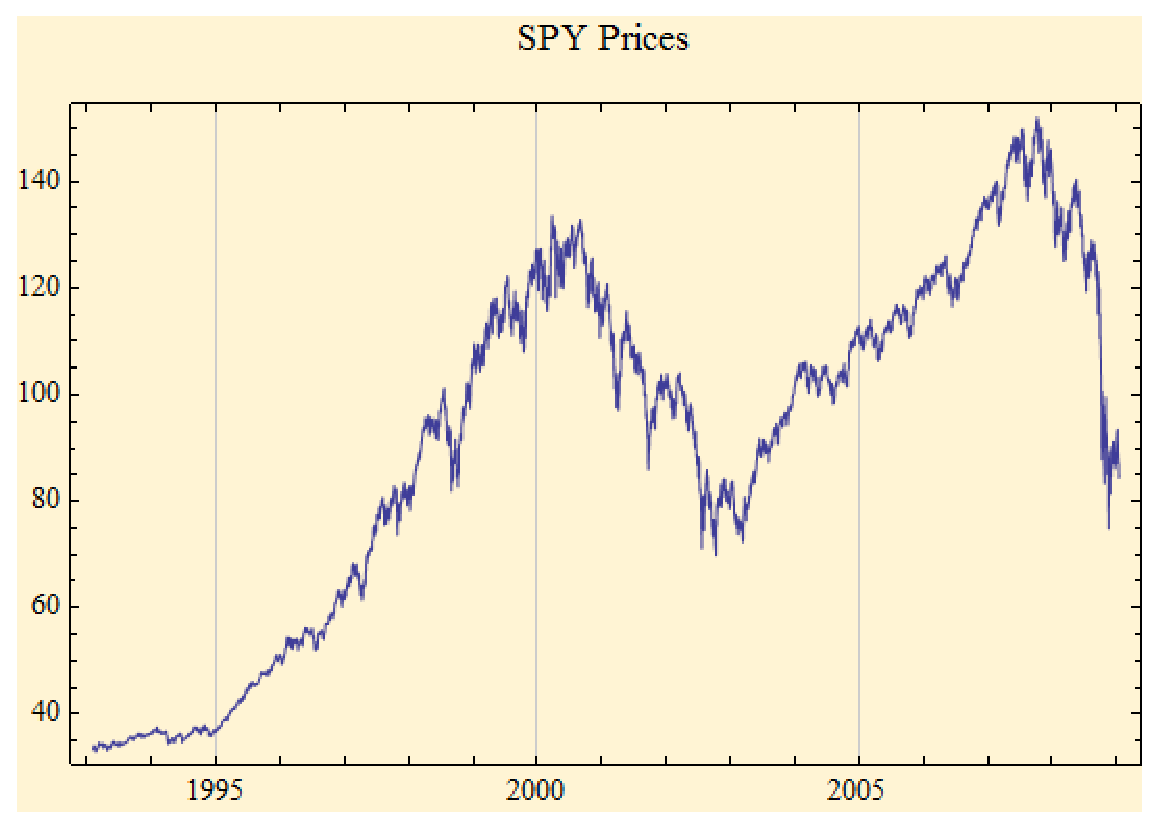
\includegraphics[width=3in]{Images/SPY.eps}
  \caption[Stock Price (ticker symbol: SPY)]
          {Stock Price (ticker symbol: SPY)}
  \label{fig:SPY}
\end{figure}

According to Nolan \cite{nolan13} a good fit of the SPY returns is achieved by a mixture of a LogNormal distribution and a Levy-Stable distribution. Using the numeric random variable facilities of RICO to plot $LogNormal(0,\sigma) \times LevyStable(\alpha, \beta, \delta, \gamma)$ for the specific fit parameters cited by Nolan \cite{nolan13},
\begin{lstlisting}
alpha = 1.86034
beta  = -0.0919429
gamma = 0.00600552
sigma = 0.532775
delta = 0.000232571
u     = log(gamma)
LN    = LogNormalNumeric(0, sigma, 100)
LS    = LevyStableNumeric(alpha, beta, delta, gamma, 100)
LNS   = LN * LS
Plot().xrange(-.1, .15).plot(LNS).show()
\end{lstlisting}

\begin{figure}
  \centering
  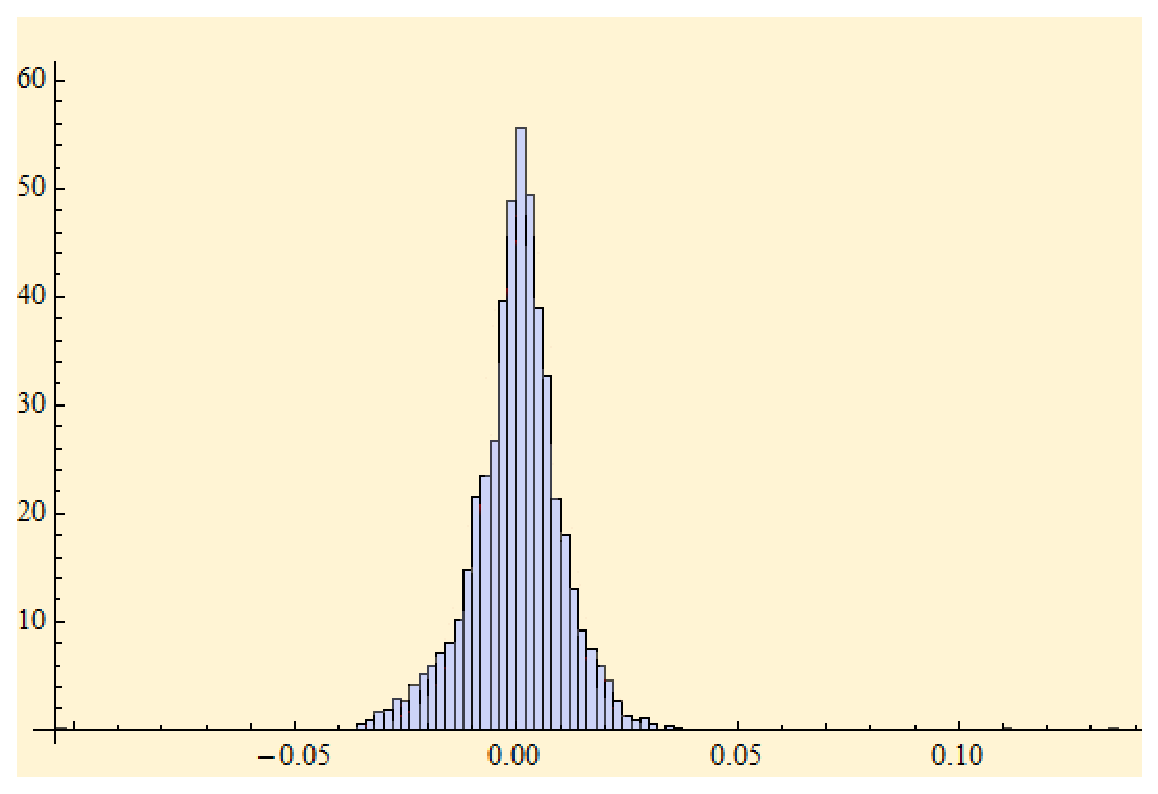
\includegraphics[width=3in]{Images/SPY_returns.eps}
  \caption[Stock Price (ticker symbol: SPY) daily return distribution]
          {Stock Price (ticker symbol: SPY) daily return distribution}
  \label{fig:SPY_returns}
\end{figure}

\begin{figure}
  \centering
  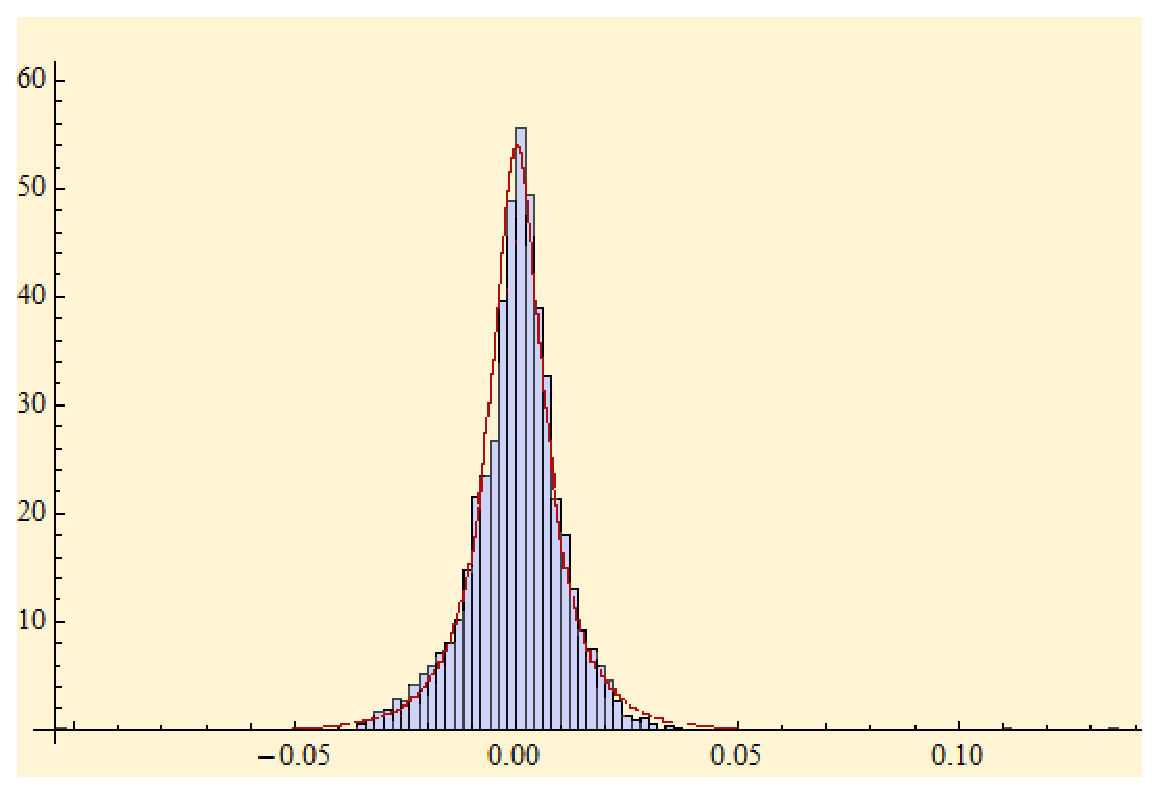
\includegraphics[width=3in]{Images/SPY_returns_fit.eps}
  \caption[Stock Price (ticker symbol: SPY) daily return distribution]
          {Stock Price (ticker symbol: SPY) daily return distribution}
  \label{fig:SPY_returns_fit}
\end{figure}

\begin{figure}
  \centering
  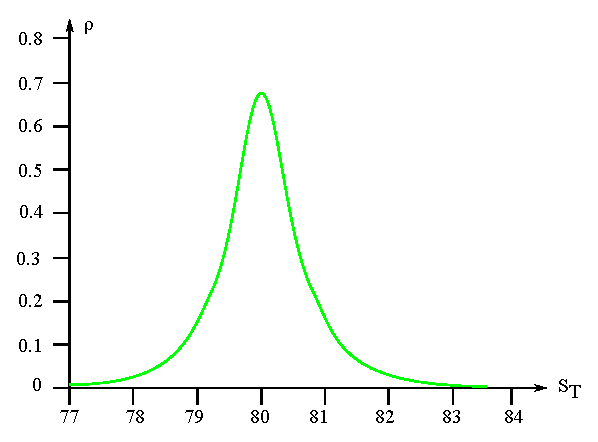
\includegraphics[width=3in]{Images/SPY_purchase.eps}
  \caption[SPY one day in future given \$80/share price today]
          {SPY one day in future given \$80/share price today}
  \label{fig:SPY_purchase}
\end{figure}

The fit found by Nolan \cite{nolan13} is overlayed on the SPY returns histogram in figure \ref{fig:SPY_returns_fit}. Suppose the current price of SPY is \$80/share. Following the Black Scholes construction, the share price of SPY at $T = $ one day in the future is denoted $S_T$ defined as,
\begin{align*}
S_T = 80 \times LNS
\end{align*}
where $LNS$ is the LogNormal-LevyStable distribution given the fit data found by Nolan \cite{nolan13}. Continuing from the previous code listing, the dsitribution of $S_T$ is computed by RICO as in the following listing with the result is shown in figure \ref{fig:SPY_purchase}.
\begin{lstlisting}
ST = 80*exp(LNS)
Plot().xrange(77,84).yrange(0,.8).plot(ST).show()
\end{lstlisting}

\begin{figure}
  \centering
  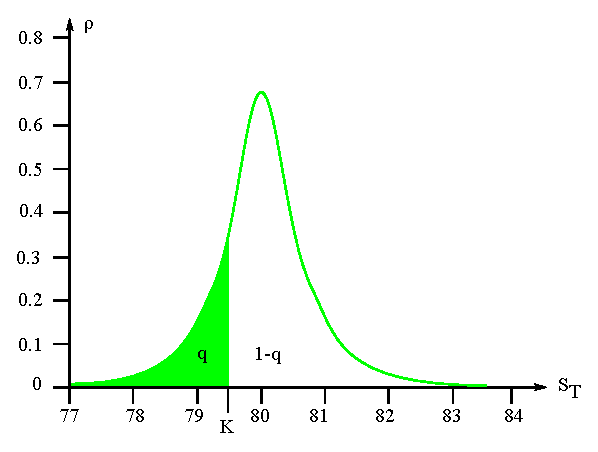
\includegraphics[width=3in]{Images/SPY_purchase_split.eps}
  \caption[SPY one day in future given \$80/share price today]
          {SPY one day in future given \$80/share price today}
  \label{fig:SPY_purchase_split}
\end{figure}

Supposing that the strike price for a 1 day option on SPY is $K = \$79.50$. The probability distribution of $S_T$ is then split at $K$ into two pieces as shown in figure \ref{fig:SPY_purchase_split}. Let
\begin{align*}
q := P(S_T < K)
\end{align*}
In this case $q \approx 0.22$ and is represented by the shaded region of figure \ref{fig:SPY_purchase_split}. The payoff random variable of a 1-day European-style call option according to the Black-Scholes construction $C_T$ is the following function of $S_T$
\begin{align*}
C_T = [S_T - K]^+
\end{align*}
shown in figure \ref{fig:SPY_purchase_call}. Notice that $C_T$ is both discrete and continuously distributed. In particular,
\begin{align*}
P(C_T = 0) = q && P(C_T > 0) = 1-q
\end{align*}

\begin{figure}
  \centering
  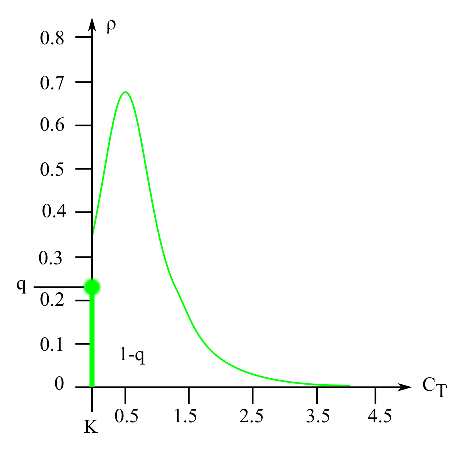
\includegraphics[width=3in]{Images/SPY_purchase_call.eps}
  \caption[Call option payoff on one-day SPY]
          {Call option payoff on one-day SPY}
  \label{fig:SPY_purchase_call}
\end{figure}

The salient point of this example is that the next step of the Black-Scholes construction cannot be completed for ths example. The reason is that the expected value of the continuous portion of $C_T$ is infinite! For the fit parameters used in this example the LNS distribution is \emph{fat tailed} and our example ends without a price for the one-day call option, $C_T$.

In practice return rates do not necessarily follow a Gaussian distribution. The Black Scholes construction remains computable so long as expected values of truncated distributions are finite. Note in particular that Monte Carlo techniques may not expose this fact.
